\documentclass[fontsize=12pt,openright,oneside,paper=a4,BCOR=1cm]{scrbook}


\newcommand{\authorname}{Felix, Wilhelm}
\newcommand{\immatriculationnumber}{78186}
\newcommand{\studypath}{Internet Computing}
\newcommand{\currentsemester}{14}
\newcommand{\email}{wilhel40@ads.uni-passau.de}
\newcommand{\worktitle}{Prozessdesign- und Digitalisierung für eine moderne Wasserwachtverwaltung}
\newcommand{\thesistype}{Bachelorarbeit}
\newcommand{\thesisdate}{20.04.2022}
\newcommand{\thesisprof}{Prof. Harald Kosch}
\newcommand{\faculty}{Fakultät für Informatik und Mathematik}
\newcommand{\chair}{Lehrstuhl für Informatik mit Schwerpunkt Verteilte Informationssysteme}
\newcommand{\semester}{14}


%%%%%%%%%%%%%%%%%%%%%%%%%%%%%%%%%%%%%%%%%%%%%%%%%%%%%%%%%%%%

% PACKAGES:


% Use list of tabels, etc. in table of contents:
\usepackage{tocbibind}
% German paragraph skip
\usepackage{parskip}
% Encoder:????
\usepackage[utf8]{inputenc}
% Index-generation
\usepackage{makeidx}
% Einbinden von URLs:
\usepackage{url}
% Include .eps-files (needed also for the CNACC-logo):
\usepackage{epsf}
% Special \LaTex symbols (e.g. \BibTeX):
\usepackage{doc}
% Include Graphic-files:
%\usepackage{graphics}
% Include Graphic-files:
\usepackage{graphicx}
% Include doc++ generated tex-files:
%\usepackage{docxx}
% Include PDF links
\usepackage{cite}
% Include citations
\usepackage{booktabs}
\usepackage{enumerate}
% figures
\usepackage{subcaption}

%mathstuff
\usepackage[cmex10]{amsmath}
\usepackage{amsfonts}
\usepackage{amssymb}

%hyperref for nice PDF output
\usepackage[pdftex, bookmarks=true]{hyperref}

%%%%%%%%%%%%%%%%%%%%%%%%%%%%%%%%%%%%%%%%%%%%%%%%%%%%%%%%%%%%

% OTHER SETTINGS:

% Pagestyle:
\pagestyle{headings}

% Chapter Format:
\addtokomafont{chapter}{\Large}
\RedeclareSectionCommand[%
  beforeskip=12pt,
  afterskip=3pt 
]{chapter}

% Avoid 'overhang':
\sloppy

% Choose language
\newcommand{\setlang}[1]{\selectlanguage{#1}\nonfrenchspacing}

\usepackage[german]{babel}


\setlang{german}

%%%%%%%%%%%%%%%%%%%%%%%%%%%%%%%%%%%%%%%%%%%%%%%%%%%%%%%%%%%%

% TITLE:

\begin{document}

%\thispagestyle{empty}
%\newpage

\vspace{1cm}

\begin{center}
\begin{tabular}{lr}

\includegraphics[width=6.5cm]{logouni.pdf}
\end{tabular}

\vspace{1.0cm}
\Large Universität Passau
\\
\Large \faculty
\\
\vspace{0.3cm}
\large \chair
\\
\vspace{0.3cm}
\large Betreuer: \thesisprof
\\


\end{center}


\vspace{1.5cm}

\begin{center}
        {\Huge \worktitle } % Master Thesis, Programming Project
\end{center}
\vspace{1.5cm}
\begin{center}

        {\LARGE Bachelorarbeit}
        \\
        {\large
        \vspace{0.3cm}
        }
        {\large
        \vspace{0.1cm}
        \thesisdate
        }
\end{center}

\vspace{0.8cm}



\vfill {% \settowidth{\baselineskip}{0.2cm}

\vfill


{\normalsize
\begin{tabular}[l]{llll}
Name:     &  \authorname \\
Matrikelnummer:       & \immatriculationnumber \\
Fachsemester:       & \currentsemester \\
Studiengang:       & \studypath \\
E-Mail Adresse:       & \email \\
\smallskip \\

\end{tabular}}
} \cleardoublepage

%%%%%%%%%%%%%%%%%%%%%%%%%%%%%%%%%%%%%%%%%%%%%%%%%%%%%%%%%%%%


% MAIN PART:

% Inhaltsverzeichnis:
\tableofcontents

%%%%%%%%%%%%%%%%%%%%%%%%%%%%%%%%%%%%
%
% Kapitel 1
%
%%%%%%%%%%%%%%%%%%%%%%%%%%%%%%%%%%%%

\chapter{Einleitung}
\section{Hintergrund und Relevanz des Themas}
Die fortschreitende Digitalisierung und Automatisierung von Verwaltungsprozessen hat in den letzten Jahren auch vor gemeinnützigen Organisationen nicht haltgemacht. Insbesondere im Bereich der Wasserwacht, die sich der Rettung von Menschenleben in und um Gewässer widmet, eröffnen moderne Informationstechnologien neue Möglichkeiten, die Effizienz von Verwaltungstätigkeiten zu steigern. Im Rahmen meiner Bachelorarbeit habe ich mich mit diesem Thema auseinandergesetzt und eine Webanwendung entwickelt, um die Verwaltungsprozesse der Wasserwacht Dingolfing-Landau zu digitalisieren. 
\\
\section{Zielsetzung der Arbeit}
Das Ziel dieser Arbeit ist es, die Herausforderungen bei der Wachplanerstellung zu identifizieren und durch den Einsatz von IT-Lösungen zu bewältigen. Dabei wird insbesondere der Prozess der Wachplanung betrachtet, der eine essenzielle Rolle in der Organisation der Wasserwacht einnimmt. Traditionell werden Wachpläne manuell erstellt, was mit einem erheblichen Zeitaufwand und administrativem Aufwand verbunden ist. Durch den Einsatz einer Webanwendung sollen diese Prozesse vereinfacht und effizienter gestaltet werden, um Zeit und Ressourcen einzusparen. 
\\
\section{Methodik und Vorgehensweise}
Im Rahmen dieser Arbeit werde ich die Anforderungen an die Webanwendung analysieren, die Technologien zur Umsetzung auswählen und die Funktionalitäten der Anwendung im Detail erläutern. Dabei werden auch Aspekte wie Datensicherheit und Benutzerfreundlichkeit berücksichtigt. Die Evaluation der entwickelten Webanwendung erfolgt anhand von Nutzertests und Feedback der Wasserwachtmitglieder, um die Praxistauglichkeit und Effektivität der Anwendung zu überprüfen. 
\\
Die vorliegende Arbeit trägt somit zur Verbesserung der Verwaltungsprozesse in der Wasserwacht bei und liefert einen Beitrag zur Nutzung moderner Informationstechnologien im gemeinnützigen Bereich. Es wird erwartet, dass die entwickelte Webanwendung die Planung und Organisation von Wacheinsätzen erleichtert und somit zur Optimierung der Einsatzbereitschaft der Wasserwacht beiträgt. 
\\


%%%%%%%%%%%%%%%%%%%%%%%%%%%%%%%%%%%%
%
% Kapitel 2
%
%%%%%%%%%%%%%%%%%%%%%%%%%%%%%%%%%%%%

%TODO
\chapter{Theoretischer Hintergrund}

\section{Wasserwacht als gemeinnützige Organisation}

\section{Verwaltungsprozesse in der Wasserwacht}

\section{Herausforderungen bei der Wachplanerstellung}

\section{Bedeutung von IT-Lösungen zur Digitalisierung von Verwaltungsprozessen} 

%TODO

%%%%%%%%%%%%%%%%%%%%%%%%%%%%%%%%%%%%
%
% Kapitel 3
%
%%%%%%%%%%%%%%%%%%%%%%%%%%%%%%%%%%%%

\chapter{Anforderungsanalyse}
\section{Identifikation von Anforderungen an die Webanwendung} 
Bevor mit der eigentlichen Implementierung der Anwendung gestartet werden kann, müssen zunächst die Anforderungen daran festgemacht werden. \\
In einem initial bereitgestelltem Dokument (sh. Anlage 1) sind die ersten Entwürfe der Anwendung aufgezeichnet. Darin sieht man mehrere gewünschte Features, um die Verwaltungsarbeiten der Wasserwacht abzudecken, wie beispielsweise "Wachplanung", "Materialcheck", "Wachbuch" oder "Sanitätsbuch". In dieser Arbeit werden hauptsächlich die Punkte "Wachplanung" und "Wachbuch" ausgearbeitet, welche im folgenden detaillierter beschrieben werden. \\ 

\subsection{Nutzergruppen}
Für die Anwendung werden zwei Nutzergruppen angefordert. \\
Zunächst hat man die "Leitungskräfte / Admins". Diese sind für administrative Tätigkeiten zuständig und erledigen die Planung und Verwaltung der Anwendung. 
Außerdem gibt es noch die "Mitglieder / Helfer". Diese spielen vor Allem bei der Durchführung der jeweiligen Wachtage eine Rolle.

\subsection{Wachplanung}
Leitungskräften soll es ermöglicht werden im Voraus Termine für die einzelnen Wachpläne einzustellen. Diese sollen für ein konkretes Datum und Uhrzeit erstellt werden können, oder als Serie mit einer bestimmten Laufzeit. In einem Kalender sollen die einzelnen Termine dargestellt werden, mit einer farblichen Kennung, ob für diesen Termin bereits Mitarbeiter eingebucht sind. \\
Für Mitglieder ist es notwendig, sich für Wachtage einzubuchen. Dazu soll auch der Kalender genutzt werden, um eine Übersicht der verfügbaren Wachtage zu erhalten.

\subsection{Wachbuch}
Im Wachbuch werden die Ereignisse eines Wachtages festgehalten. Nutzern soll es möglich sein, eine Liste der gebuchten Helfern anzuzeigen, sowie nach Wachstart eine Liste der anwesenden Helfern anzuzeigen. Nutzer können sich für diesen Wachtag ein-, bzw. ausbuchen. \\
Weiterhin werden für diesen Wachtag die vorliegenden Wetterdaten vorliegen, welche über eine API ermittelt werden. Nutzer können die aktuelle Wassertemperatur über ein Eingabefeld abspeichern. \\
Die Ereignisse des Wachtags werden in einer Tabelle, mit Namen und Zeitstempel, festgehalten. Dabei werden der Wachbeginn und das Wachende der Mitglieder, die An- und Abmeldung im ILS, die automatischen Wetterdaten und der Wachstart/ -ende automatisch eingetragen. Nutzer können zusätzlich manuell Eingaben tätigen. \\
Leitungskräften soll es zusätzlich ermöglicht werden eine Auswertung eines Wachtages vorzunehmen. Dazu gibt es einen Button "Drucken", über den ein PDF, welches die Ereignisse des Wachtages zusammenfasst, heruntergeladen werden kann. Die Informationen, welche dieses Dokument enthalten muss, wurden aus einem derzeit verwendeten Wachbuch übernommen (sh. Anlage 2). Darin befinden sich die vorliegenden Wetterdaten, Informationen über das anwesende Wachpersonal, sowie das Wachtagebuch. \\
Die Punkte "Übersicht Checks" und "Einsätze" wurden im Rahmen dieser Arbeit nicht betrachtet. 

\section{Befragung von Wasserwachtmitgliedern und Mockups}
In mehreren Iterationen wurden mit Herrn Andreas Schmeisl (Vorsitzender Kreiswasserwacht Dingolfing-Landau) und Herrn Werner Gerl (Technischer Leiter) die finalen Vorgaben geklärt. Dabei wurde mit Hilfe von Mockups ein Zielbild der Anwendung entwickelt. 
\subsection{Mockups}
\subsubsection{Was sind Mockups}
%Definition Mockups, warum werden sie in der Planung von Software eingesetzt
Mockups werden in der Softwareentwicklung eingesetzt um sicher zu gehen, dass man die Anforderungen an die Anwendung verstanden hat. Mockups haben den Vorteil, dass sie kosten- und zeiteffizient erstellt werden können und schnell anpassbar sind.

\subsubsection{Papier-Mockups}
In einem initialen Meeting wurden mit Papier Mockups die groben Umrisse der Website aufgezeigt. Es wurden außerdem noch weitere Funktionalitäten und Anforderungen besprochen, die aus den vorliegenden Unterlagen nicht hervorgingen. \\
Mit den Ergebnissen aus diesem Meeting konnte ein Prototyp der Anwendung erstellt werden.


\subsubsection{Figma}
%Website beschreiben 
Figma ist eine Website, über die man Protoypen und Mockups erstellen kann. Über einzelne Boards können die verschiedenen Seiten der Zielanwendung simuliert werden. Der Vorteil hierbei ist, dass auch Nutzereingaben simuliert werden können. So kann beispielsweise bei Klicken ein Seitensprung animiert werden. Dadurch kann man ohne viel Aufwand dem Kunden zeigen, wie die Anwendung einmal aussehen wird. 

\subsection{Ergebnisse}
%Bilder der Mocks darstellen, einzelne Masken wurden konkretisiert, weitere Anforderungen wurden aufgenommen, Emailversand bei Login. 
Mit Figma wurden alle vorgesehenen Seiten der Website dargestellt. Dabei kamen noch weitere Anforderungen auf: \\
Beim Login Prozess wurde gefordert, dass die "Admins" bei einer Neu-Anmeldung über Email benachrichtigt werden. Neue Nutzer können daher nach dem registrieren nicht sofort auf die Seite zugreifen, sondern müssen erst warten bis ein Admin sie bestätigt hat.\\

\begin{figure}[h!]
  \centering
  \begin{subfigure}[b]{0.4\linewidth}
    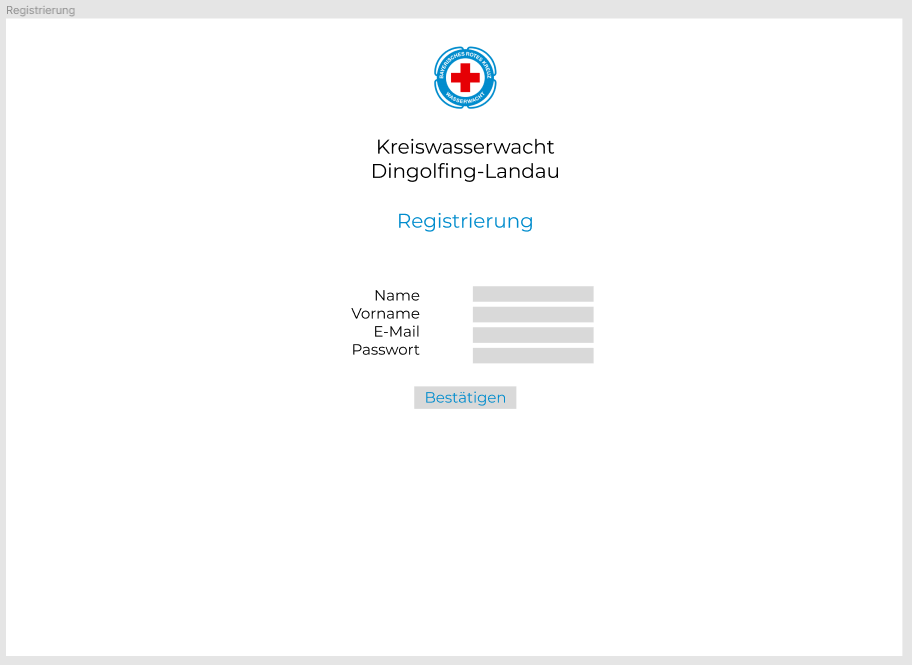
\includegraphics[width=\linewidth]{Anlagen/Figma/2-Registrierung.png}
    \caption{Registrierung}
  \end{subfigure}
  \begin{subfigure}[b]{0.4\linewidth}
    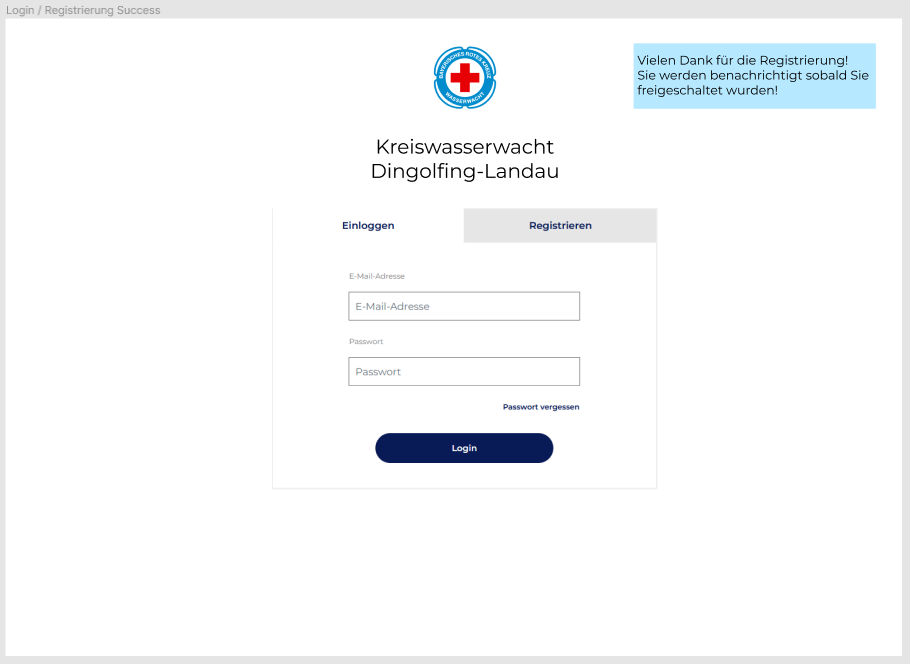
\includegraphics[width=\linewidth]{Anlagen/Figma/3-LoginSuccess.png}
    \caption{Benachrichtigung nach Registrierung}
  \end{subfigure}
  \caption{AnmeldeProzess}
  \label{fig:anmeldeprozess}
\end{figure}

Admins sehen auf der Nutzerübersicht alle Nutzer und ob sie bereits freigeschaltet wurden. Über das jeweilige Nutzerprofil können sie den Nutzer über einen Button freischalten. Danach wird der Nutzer per Email benachrichtigt und erhält Zugang zum System. \\

\begin{figure}[h!]
  \centering
  \begin{subfigure}[b]{0.4\linewidth}
    \includegraphics[width=\linewidth]{Anlagen/Figma/6-Nutzerübersicht.png}
    \caption{Nutzerübersicht}
  \end{subfigure}
  \begin{subfigure}[b]{0.4\linewidth}
    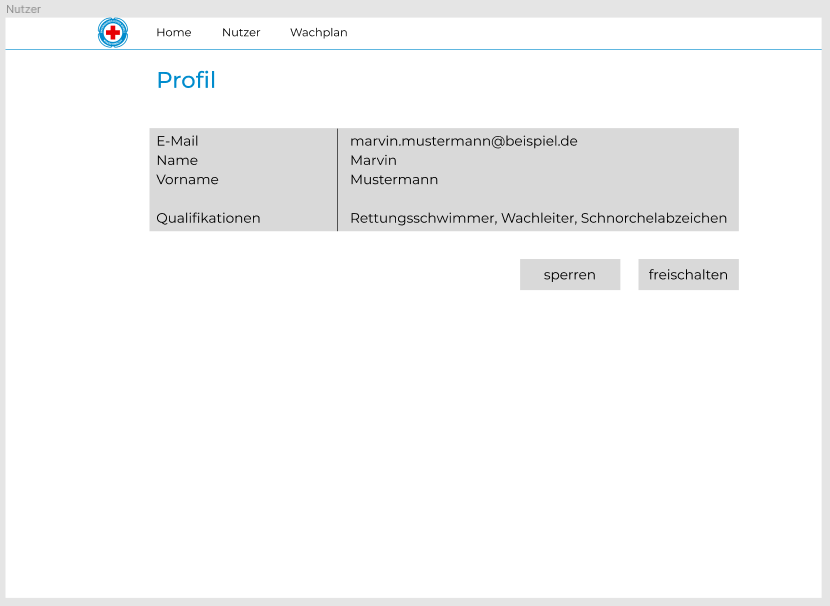
\includegraphics[width=\linewidth]{Anlagen/Figma/7-ProfilAdminSicht.png}
    \caption{Profil Admin Ansicht}
  \end{subfigure}
  \caption{Freischaltungs-Prozess}
  \label{fig:freischaltprozess}
\end{figure}

Bei der Wachplanung wurde angefordert, dass Wachtermine einzeln für ein bestimmtes Datum und Uhrzeit angelegt werden können. Außerdem soll es möglich sein gleich eine Reihe an Terminen anzulegen. Dazu muss ein Start- und Enddatum angegeben werden, die Uhrzeit, sowie die Wochentage an denen ein Termin eingestellt werden soll. Als Übersicht für die bisherigen Termine wird ein Kalender verwendet. Hier wurde überlegt, ob man die einzelnen Termine farbig codiert, wenn beispielsweise ein "Rettungsschwimmer" und "Wachleiter" noch nicht eingebucht sind. In weiteren Abstimmungsterminen hat man sich aber darauf geeinigt, die Termine rot einzufärben, wenn noch niemand eingebucht ist, und grün einzufärben wenn Nutzer eingebucht sind (vgl. \cite[S. 49]{sklar2011principles}).


%%%%%%%%%%%%%%%%%%%%%%%%%%%%%%%%%%%%
%
% Kapitel 4
%
%%%%%%%%%%%%%%%%%%%%%%%%%%%%%%%%%%%%
\renewcommand{\cleardoublepage}{}
\chapter{Technologien und Methoden}

\section{Auswahl geeigneter Technologien und Tools für die Webanwendung}

\section{Beschreibung der verwendeten Programmiersprachen, Frameworks und Datenbanken}

\subsection{Spring}

\subsection{Thymeleaf}

\subsection{Postgres}

\subsection{Wetter API}

\section{Agile Entwicklungsmethoden zur Umsetzung des Projekts}


%%%%%%%%%%%%%%%%%%%%%%%%%%%%%%%%%%%%
%
% Kapitel 5
%
%%%%%%%%%%%%%%%%%%%%%%%%%%%%%%%%%%%%

\renewcommand{\cleardoublepage}{}
\chapter{Konzeption und Umsetzung}

\section{Detaillierte Beschreibung der Konzeption der Webanwendung}

\subsection{Datenmodell}
\subsection{Prozesse}

\section{Funktionalitäten und Features der Anwendung}

\section{Umsetzung der Webanwendung anhand von Best Practises}


%%%%%%%%%%%%%%%%%%%%%%%%%%%%%%%%%%%%
%
% Kapitel 6
%
%%%%%%%%%%%%%%%%%%%%%%%%%%%%%%%%%%%%

\renewcommand{\cleardoublepage}{}
\chapter{Evaluation}

\section{Nutzertests und Feedback der Wasserwachtmitglieder}

\section{Bewertung der Praxistauglichkeit und Effektivität der Webanwendung}

\section{Klickmetriken}

\section{Verbesserungspotentiale}

%%%%%%%%%%%%%%%%%%%%%%%%%%%%%%%%%%%%
%
% Kapitel 7
%
%%%%%%%%%%%%%%%%%%%%%%%%%%%%%%%%%%%%

\renewcommand{\cleardoublepage}{}
\chapter{Ergebnisse und Diskussion}

\section{Zusammenfassung der Ergebnisse}

\section{Diskussion der Erkenntnisse im Kontext der Zielsetzung der Arbeit}

\section{Ausblick auf zukünftige Entwicklungen und mögliche Erweiterungen der Webanwendung}

%%%%%%%%%%%%%%%%%%%%%%%%%%%%%%%%%%%%
%
% Kapitel 8
%
%%%%%%%%%%%%%%%%%%%%%%%%%%%%%%%%%%%%

\renewcommand{\cleardoublepage}{}
\chapter{Fazit}

\section{Zusammenfassung der Arbeit}

\section{Beantwortung der Forschungsfrage}

\section{Schlussfolgerungen und Handlungsempfehlungen}


% References (Literaturverzeichnis):
\bibliographystyle{alpha}
\bibliography{Literatur}


%%%%%%%%%%%%%%%%%%%%%%%%%%%%%%%%%%%%%%%%%%%%%%%%%%%%%%%%%%%%
\end{document}
